\section{Python control system packages.}

In this chapter some advance python control and optimization packages will be discussed.

The first one is \textbf{python Control Systems} Library v0.84 \cite{Control_Lib} \cite{GitControl_Lib} with the last update on 16/03/2021 (the day when this report is written).

The main features are: 

\begin{itemize}
    \item Linear input/output systems in state-space and frequency domain

    \item Nonlinear input/output system modeling, simulation, and analysis

    \item Block diagram algebra: serial, parallel, and feedback interconnections

    \item Time response: initial, step, impulse

    \item Frequency response: Bode and Nyquist plots

    \item Control analysis: stability, reachability, observability, stability margins

    \item Control design: eigenvalue placement, LQR, H2, Hinf, MPC

    \item Model reduction: balanced realizations, Hankel singular values

    \item Estimator design: linear quadratic estimator (Kalman filter)
    
    \item The optimal control module with optimization based controllers for nonlinear systems with state and input constraints.

\end{itemize}

Another python package for machine learning and optimization is \textbf{GEKKO Optimization Suite}\cite{gekko2018}. It is coupled with large-scale solvers for linear, quadratic, nonlinear, and mixed integer programming (LP, QP, NLP, MILP, MINLP). Modes of operation include parameter regression, data reconciliation, real-time optimization, dynamic simulation, and nonlinear predictive control. The paper release with the package has been selected as a 2020 Best Paper by the journal Processes (figure: \ref{figure:Gekko}). 

\begin{figure}[H]
	\centering
	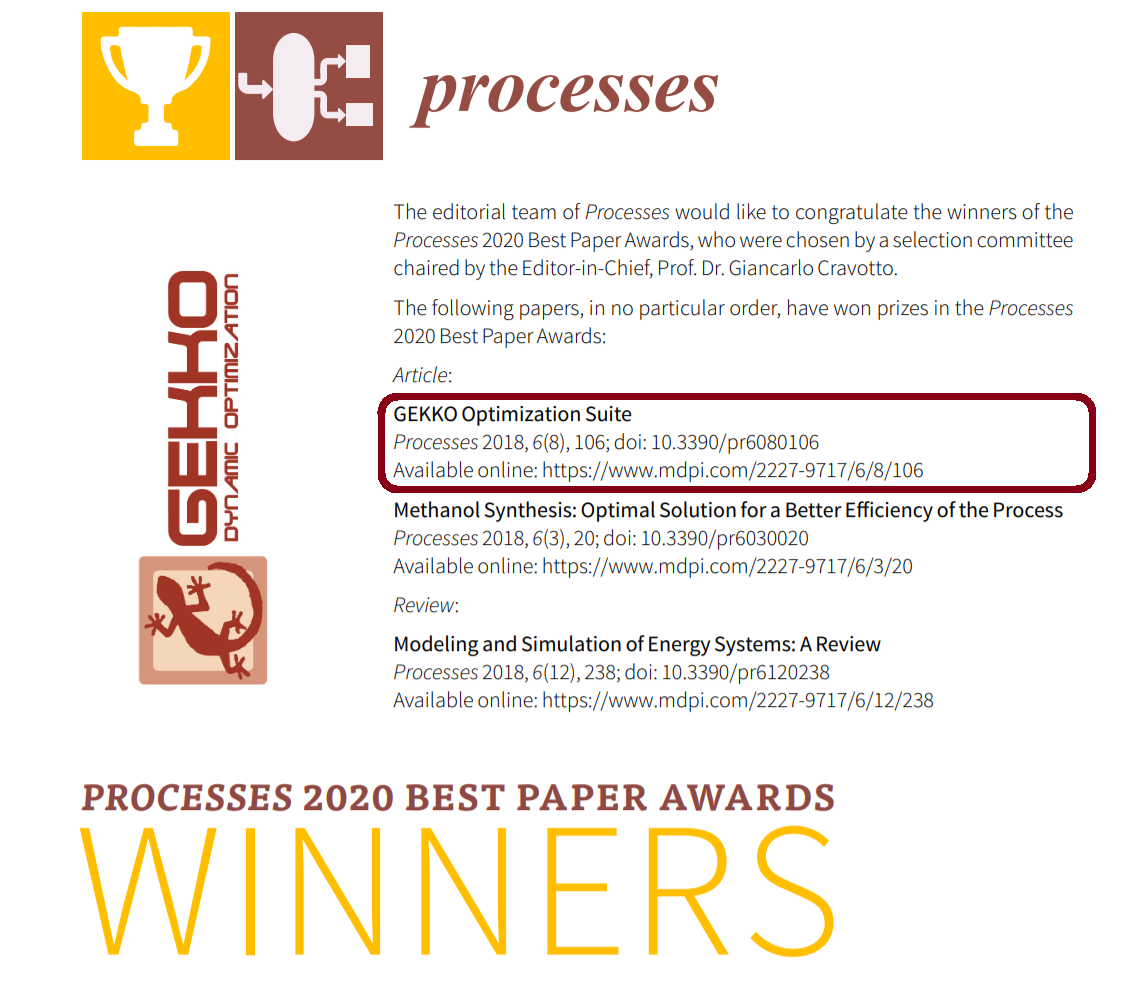
\includegraphics[width=0.8\columnwidth]{Pictures/gekko_best_paper2020.png}
	\caption[Short title]{Gekko best paper award 2020}
	\label{figure:Gekko}
\end{figure}

 Beside the 2 python packages which have been mentioned above there is a collection of Jupiter python/notebook series on optimization and control CBE 30338 (figure \ref{figure:CBE}) and CBE 32338 (\ref{figure:CBE_Lab}) Chemical Process Control \cite{CBE} \cite{CBE_Lab}. The notebooks series contain a lot of python example on optimization technique. For example, the linear programming has been mentioned in section 6.3 \cite{CBE} CBE 30338 (\ref{figure:CBE}) and the model predictive control in section 5.1, 5.2 \cite{CBE_Lab} CBE 32338 (\ref{figure:CBE_Lab}) 

\begin{figure}[H]
	\centering
	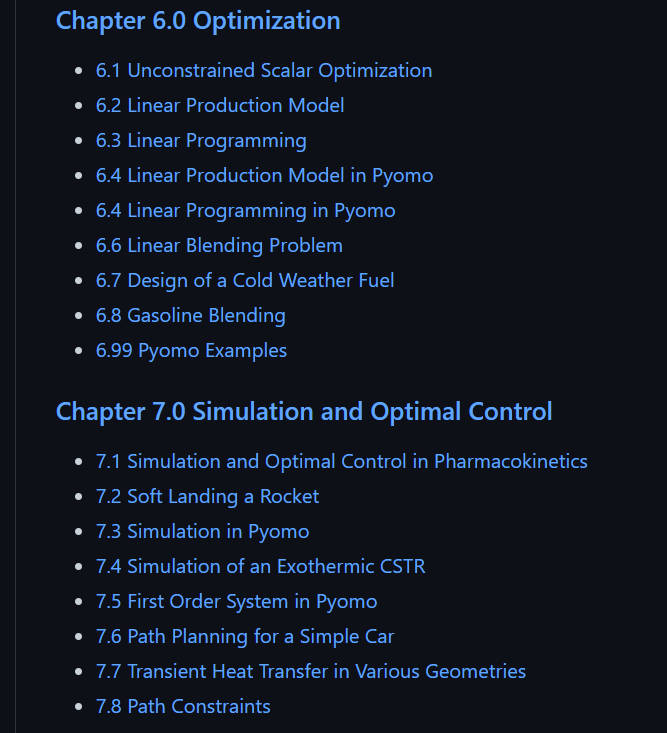
\includegraphics[width=0.8\columnwidth]{Pictures/Optimization_CBE.png}
	\caption[Short title]{CBE 30338 Chemical Process Control}
	\label{figure:CBE}
\end{figure}

\begin{figure}[H]
	\centering
	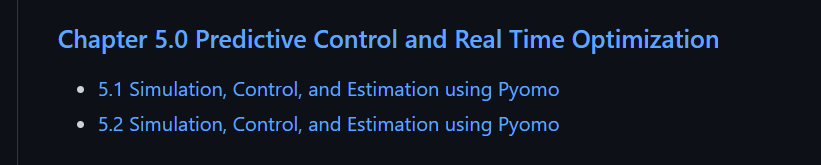
\includegraphics[width=0.8\columnwidth]{Pictures/Optimization_CBE_Lab.png}
	\caption[Short title]{CBE 32338 Process Control Laboratory}
	\label{figure:CBE_Lab}
\end{figure}

\newpage
	
	
